% ============================================================
% 20_tables.tex — Tabellen-Helfer (semantisches Table-System)
% ============================================================
% Zentrales Design-Prinzip:
%   1. Tabellen fuellen IMMER \linewidth (kein manuelles p{0.16..}).
%   2. Spaltenbreiten werden PROPORTIONAL deklariert (Y{0.18} L{0.54} ...),
%      sodass die Summe der Faktoren = Anzahl X-Spalten ergibt.
%   3. Zebra-Streifen + Header-Highlight sind ins Environment eingebaut;
%      direkte Farb-Primitive sind in Kapiteln per Linter verboten.
%
% Damit ist strukturell ausgeschlossen:
%   - zu kurze Zebra-Streifen (Tabelle schmaler als Box),
%   - überstehende Zeilen (Content sprengt Box-Breite),
%   - Drift zwischen Kapiteln (jede Tabelle nutzt dieselben Wrapper).

% ------------------------------------------------------------
% Spaltentypen (tabularx-X-Varianten)
% ------------------------------------------------------------
% Feste Varianten — jede zaehlt als Faktor 1:
% m{#1}: X-Spalten vertikal mittig (Text + Grafik in einer Zeile).
\setlength{\extrarowheight}{3pt}
\renewcommand{\arraystretch}{1.25}

\renewcommand{\tabularxcolumn}[1]{m{#1}}
\newcolumntype{L}{>{\RaggedRight\arraybackslash}X}   % linksbuendig, umbricht
\newcolumntype{C}{>{\Centering\arraybackslash}X}     % zentriert,  umbricht
\newcolumntype{R}{>{\RaggedLeft\arraybackslash}X}    % rechtsbuendig, umbricht

% Parametrisierte, proportionale Varianten — #1 = relativer Anteil.
%
% WICHTIG (tabularx-Konvention): Die Summe aller Faktoren in EINER
% Tabelle muss = Anzahl X-Spalten sein, damit die Tabelle \linewidth
% voll ausfuellt. L/C/R zählen als Faktor 1.
%
% Beispiele (2 Spalten → Summe 2):
%   Y{0.6}  Y{1.4}            → 30% / 70%
%   Y{1}    Y{1}              → 50% / 50% (== L L)
%   Q{0.8}  Y{1.2}            → 40% / 60%, Spalte 1 rechtsbuendig
% Beispiele (3 Spalten → Summe 3):
%   Y{0.6}  Y{1.5}  Y{0.9}    → 20% / 50% / 30%
%   L       Y{2}    L         → 25% / 50% / 25%
% Beispiele (4 Spalten → Summe 4):
%   Y{1.2}  Y{0.8}  Y{1.2}  Y{0.8}  → 30% / 20% / 30% / 20%
\newcolumntype{Y}[1]{>{\hsize=#1\hsize\RaggedRight\arraybackslash}X} % linksb., proport.
\newcolumntype{Z}[1]{>{\hsize=#1\hsize\Centering\arraybackslash}X}   % zentriert, proport.
\newcolumntype{Q}[1]{>{\hsize=#1\hsize\RaggedLeft\arraybackslash}X}  % rechtsb., proport.

% Zentrierte Formel-Spalte (Math-Mode automatisch, proportional)
\newcolumntype{F}[1]{>{\hsize=#1\hsize\Centering\arraybackslash$}X<{$}}

% ------------------------------------------------------------
% Zebra-Streifen (Scannbarkeit)
% ------------------------------------------------------------
\newcommand{\ZSFzebraBG}{\chaptercolorlight!70}
\newcommand{\SetZSFzebraBG}[1]{\renewcommand{\ZSFzebraBG}{#1}}
\newcommand{\ZSFzebra}{\rowcolors{2}{white}{\ZSFzebraBG}}          % Header in Zeile 1
\newcommand{\ZSFzebraStart}[1]{\rowcolors{#1}{white}{\ZSFzebraBG}} % frei wählbar
\newcommand{\ZSFzebraOff}{\rowcolors{1}{}{}}

% ------------------------------------------------------------
% Header-Highlight
% ------------------------------------------------------------
% Konvention:
%   \ZSFheaderRow   — startet die Header-Zeile und setzt den Zeilen-Hintergrund.
%   \ZSFhead{<Text>} — umschliesst den Inhalt JEDER Header-Zelle (Farbe + bold).
%
% Warum zweigeteilt? In tabularx-X-Spalten propagiert \color, das direkt nach
% \rowcolor am Zeilenanfang gesetzt wird, NICHT zuverlässig über die
% &-Grenzen. Die erste Zelle verliert die Farbe, andere behalten sie — je
% nach Spaltenbreite und Content (siehe SI-Praefix-Bug). Per-Zelle-Wrapper
% via \ZSFhead{...} ist robust und konsistent.
\newcommand{\ZSFheaderRowBG}{\chaptercolor}
\newcommand{\ZSFheaderRowFG}{\chaptercolortext}
\newcommand{\ZSFheaderRow}{\rowcolor{\ZSFheaderRowBG}}
\newcommand{\ZSFhead}[1]{{\color{\ZSFheaderRowFG}\bfseries\ZSFVariableColorsOff #1}}

% Strut für Tabellenzeilen mit grossen Formeln (z.B. \dfrac), um Berührung mit Linien/Hintergründen zu verhindern
\newcommand{\ZSFtablestrut}{\rule[-8pt]{0pt}{19pt}}

% ------------------------------------------------------------
% Semantische Tabellen-Environments (Single Point of Truth)
% ------------------------------------------------------------
% Signatur (alle drei Varianten):
%   \begin{ZSFtable}[<font>]{<colspec>}       -- Header + Zebra ab Zeile 2
%   \begin{ZSFtableFlat}[<font>]{<colspec>}   -- kein Header, Zebra ab Zeile 1
%   \begin{ZSFtablePlain}[<font>]{<colspec>}  -- ohne Zebra
%
% <font> ist OPTIONAL und ein semantisches Font-Makro aus
% styles/50_typography_semantics.tex:
%   - \ZSFfontTable        (Default, \normalsize)
%   - \ZSFfontTableDense   (\footnotesize — für lange/dichte Tabellen)
%
% colspec nutzt L/C/R (gleichverteilt, jeweils Faktor 1) oder
% Y{.}/Z{.}/Q{.}/F{.} (proportional). Summe der Faktoren muss gleich
% der Anzahl X-Spalten sein (tabularx-Konvention).
%
% Beispiel:
%   \begin{ZSFtable}[\ZSFfontTableDense]{Y{0.6} Y{1.55} Y{0.85}}
%     \ZSFheaderRow \ZSFhead{Symbol} & \ZSFhead{Bedeutung} & \ZSFhead{SI-Einheit} \\
%     $e$ & Elementarladung & \si{C} \\
%     ...
%   \end{ZSFtable}

\NewDocumentEnvironment{ZSFtable}{O{\ZSFfontTable} m}{%
  #1%
  \ZSFzebra
  \tabularx{\linewidth}{#2}%
}{%
  \endtabularx
}

\NewDocumentEnvironment{ZSFtableFlat}{O{\ZSFfontTable} m}{%
  #1%
  \ZSFzebraStart{1}%
  \tabularx{\linewidth}{#2}%
}{%
  \endtabularx
}

% Reine Tabelle ohne Zebra (selten; für einspaltige Zebraschäden etc.)
\NewDocumentEnvironment{ZSFtablePlain}{O{\ZSFfontTable} m}{%
  #1%
  \ZSFzebraOff
  \tabularx{\linewidth}{#2}%
}{%
  \endtabularx
}

% ------------------------------------------------------------
% Ampel-Hinterlegung (0..4) für Eignungstabellen (WNV, Lager etc.)
% ------------------------------------------------------------
\definecolor{MKeigNull}{HTML}{F9C9C4}%  0 = helles Rot
\definecolor{MKeigEins}{HTML}{FBDCB6}%  1 = helles Orange
\definecolor{MKeigZwei}{HTML}{FAF0B4}%  2 = helles Gelb
\definecolor{MKeigDrei}{HTML}{D6EFC4}%  3 = helles Grün
\definecolor{MKeigVier}{HTML}{A9DEA0}%  4 = etwas dunkleres helles Grün

\newcommand{\MKlvl}[2]{%
  \ifcase#1\relax
    \cellcolor{MKeigNull}#2\or\cellcolor{MKeigEins}#2\or\cellcolor{MKeigZwei}#2%
    \or\cellcolor{MKeigDrei}#2\or\cellcolor{MKeigVier}#2\fi}
\newcommand{\MKeig}[1]{\MKlvl{#1}{#1}}

\newcommand{\MKeigLeg}[2]{%
  \itshape\color{black!60}\begin{tabular}[b]{@{}c@{}}%
  \colorbox{MKeigVier}{\color{black!75}(4)} #1\\[0.4pt]
  \colorbox{MKeigDrei}{\rule{0pt}{3.6pt}\,}\colorbox{MKeigZwei}{\rule{0pt}{3.6pt}\,}\colorbox{MKeigEins}{\rule{0pt}{3.6pt}\,}\\[0.4pt]
  \colorbox{MKeigNull}{\color{black!75}(0)} #2\end{tabular}}

\newcommand{\zsfWNh}[1]{\rotatebox{90}{\,#1\,}}
\newcommand{\zsfWNhh}[2]{\rotatebox{90}{\,{\renewcommand{\arraystretch}{0.78}\begin{tabular}{@{}l@{}}#1\\ #2\end{tabular}}\,}}

\newcommand{\ZSFReibschlussFormschlussTabelle}{%
  {\centering\noindent\hspace*{-\ZSFspaceM}%
  {\sffamily\ZSFfontRel{-3.5bp}{0.4bp}%
  \setlength{\tabcolsep}{0.7pt}%
  \renewcommand{\arraystretch}{1.02}%
  \arrayrulecolor{black!35}%
  \begin{tabular}{|>{\columncolor{black!8}}l|*{9}{c|}c!{\color{black!65}\vrule width 1.1pt}*{6}{c|}}
  \hline
  \multicolumn{1}{|l|}{} & \multicolumn{10}{c!{\color{black!65}\vrule width 1.1pt}}{\cellcolor{black!12}\textbf{Reibschluss}} & \multicolumn{6}{c|}{\cellcolor{black!12}\textbf{Formschluss}}\\
  \hline
  \multicolumn{1}{|c|}{\MKeigLeg{sehr gut}{ungeeignet}} &
  \zsfWNhh{Zylindrischer}{Pressverband} &
  \zsfWNhh{Kegelpressverband}{(teuer)} &
  \zsfWNhh{Kegelspann-}{elemente} &
  \zsfWNh{Kegelspannsatz} &
  \zsfWNhh{Schrumpfscheibe}{(Schraube)} &
  \zsfWNh{Sternscheiben} &
  \zsfWNh{Druckh\"ulse} &
  \zsfWNh{Toleranzring} &
  \zsfWNh{Klemmverb.} &
  \zsfWNhh{Kreiskeil-}{verb.} &
  \zsfWNh{Passfeder} &
  \zsfWNh{Keilwelle} &
  \zsfWNh{Zahnwelle} &
  \zsfWNh{Polygonprofil} &
  \zsfWNh{L\"angsstift} &
  \zsfWNh{Querstift}\\
  \hline
  Grosses \textbf{einseitiges} Drehmom. & \MKeig{4} & \MKeig{4} & \MKeig{3} & \MKeig{4} & \MKeig{4} & \MKeig{2} & \MKeig{3} & \MKeig{0} & \MKeig{2} & \MKeig{4} & \MKeig{2} & \MKeig{4} & \MKeig{4} & \MKeig{4} & \MKeig{2} & \MKeig{1} \\
  \hline
  \quad $\cdot$ auch \textbf{wechselndes/stosshaftes} Drehmom. & \MKeig{4} & \MKeig{4} & \MKeig{3} & \MKeig{4} & \MKeig{4} & \MKeig{2} & \MKeig{3} & \MKeig{0} & \MKeig{2} & \MKeig{3} & \MKeig{2} & \MKeig{3} & \MKeig{3} & \MKeig{4} & \MKeig{0} & \MKeig{0} \\
  \hline
  Aufnahme Ax.-kr\"afte$\uparrow$ & \MKeig{4} & \MKeig{4} & \MKeig{2} & \MKeig{3} & \MKeig{3} & \MKeig{2} & \MKeig{3} & \MKeig{1} & \MKeig{2} & \MKeig{4} & \MKeig{0} & \MKeig{0} & \MKeig{0} & \MKeig{0} & \MKeig{0} & \MKeig{1} \\
  \hline
  Nabe ax.\ verschiebbar & \MKeig{0} & \MKeig{0} & \MKeig{0} & \MKeig{0} & \MKeig{0} & \MKeig{0} & \MKeig{0} & \MKeig{0} & \MKeig{0} & \MKeig{2} & \MKeig{4} & \MKeig{4} & \MKeig{2} & \MKeig{2} & \MKeig{0} & \MKeig{0} \\
  \hline
  Nabe in Drehrichtung versetzbar & \MKeig{3} & \MKeig{4} & \MKeig{4} & \MKeig{4} & \MKeig{4} & \MKeig{4} & \MKeig{4} & \MKeig{4} & \MKeig{4} & \MKeig{0} & \MKeig{0} & \MKeig{2} & \MKeig{2} & \MKeig{2} & \MKeig{0} & \MKeig{0} \\
  \hline
  Max. übertragbares Drehmom.\ \textbf{nachstellbar} & \MKeig{0} & \MKeig{4} & \MKeig{4} & \MKeig{4} & \MKeig{4} & \MKeig{4} & \MKeig{0} & \MKeig{4} & \MKeig{4} & \MKeig{3} & \MKeig{0} & \MKeig{0} & \MKeig{0} & \MKeig{0} & \MKeig{0} & \MKeig{0} \\
  \hline
  Fertigungsaufwand$\downarrow$ & \MKeig{4} & \MKeig{2} & \MKeig{2} & \MKeig{2} & \MKeig{2} & \MKeig{3} & \MKeig{4} & \MKeig{4} & \MKeig{2} & \MKeig{1} & \MKeig{3} & \MKeig{1} & \MKeig{1} & \MKeig{1} & \MKeig{2} & \MKeig{2} \\
  \hline
  Montageaufwand$\downarrow$ & \MKeig{2} & \MKeig{4} & \MKeig{4} & \MKeig{4} & \MKeig{4} & \MKeig{4} & \MKeig{4} & \MKeig{4} & \MKeig{3} & \MKeig{4} & \MKeig{3} & \MKeig{3} & \MKeig{3} & \MKeig{3} & \MKeig{3} & \MKeig{4} \\
  \hline
  Gute Wiederverwendbarkeit & \MKeig{1} & \MKeig{4} & \MKeig{4} & \MKeig{4} & \MKeig{4} & \MKeig{4} & \MKeig{4} & \MKeig{4} & \MKeig{4} & \MKeig{3} & \MKeig{4} & \MKeig{4} & \MKeig{4} & \MKeig{4} & \MKeig{2} & \MKeig{2} \\
  \hline
  Selbstzentr. & \MKeig{4} & \MKeig{4} & \MKeig{0} & \MKeig{4} & \MKeig{4} & \MKeig{0} & \MKeig{4} & \MKeig{0} & \MKeig{2} & \MKeig{3} & \MKeig{3} & \MKeig{4} & \MKeig{4} & \MKeig{4} & \MKeig{4} & \MKeig{4} \\
  \hline
  Unwucht$\downarrow$ $\Rightarrow$ \textbf{Drehz.$\uparrow$} ok & \MKeig{4} & \MKeig{4} & \MKeig{2} & \MKeig{3} & \MKeig{3} & \MKeig{1} & \MKeig{3} & \MKeig{0} & \MKeig{0} & \MKeig{3} & \MKeig{2} & \MKeig{3} & \MKeig{3} & \MKeig{4} & \MKeig{1} & \MKeig{1} \\
  \hline
  Kerbwirkung$\downarrow$ auf Welle & \MKeig{1} & \MKeig{2} & \MKeig{2} & \MKeig{3} & \MKeig{3} & \MKeig{2} & \MKeig{2} & \MKeig{4} & \MKeig{1} & \MKeig{1} & \MKeig{1} & \MKeig{1} & \MKeig{1} & \MKeig{1} & \MKeig{1} & \MKeig{0} \\
  \hline
  \end{tabular}%
  \arrayrulecolor{black}}%
  \hspace*{-\ZSFspaceM}\par}
}

\newcommand{\MKrfIcon}[1]{\raisebox{-0.25\height}{\includegraphics[height=8bp,keepaspectratio]{graphics/#1.pdf}}}

\newcommand{\ZSFKupplungenDrehsteifTabelle}{%
  {\setlength{\tabcolsep}{0.8pt}%
  \arrayrulecolor{black!35}%
  \begin{ZSFtablePlain}[\ZSFfontRel{-3bp}{0.3bp}]{|>{\columncolor{black!8}}Z{0.9}|>{\columncolor{black!8}}Z{1.42}|Z{0.98}|Z{0.95}|Z{0.9}|Z{0.9}|Z{0.95}|}
  \hline
  \ZSFheaderRow \ZSFhead{} & \ZSFhead{Kupplung} & \ZSFhead{Drehmom.} & \ZSFhead{Drehz.} & \multicolumn{3}{c|}{\ZSFhead{Versatz-Ausgleich}} \\
  \ZSFheaderRow \ZSFhead{} & \ZSFhead{} & \ZSFhead{} & \ZSFhead{} & \ZSFhead{axial} & \ZSFhead{radial} & \ZSFhead{winklig} \\
  \noalign{\global\arrayrulewidth=1.1pt}\hline\noalign{\global\arrayrulewidth=0.4pt}%
  \multicolumn{7}{|l|}{\cellcolor{white}\MKrfIcon{icon_drehsteif}\ \textbf{Drehsteif}{\color{black!60}: winkelsynchron, keine Dämpfung}} \\
  \noalign{\global\arrayrulewidth=1.1pt}\hline\noalign{\global\arrayrulewidth=0.4pt}%
  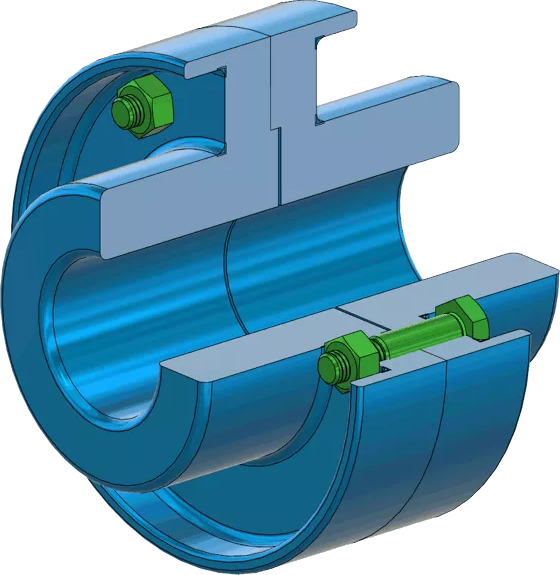
\includegraphics[width=0.68cm,height=0.6cm,keepaspectratio]{graphics/scheibenkupplung.png} & Scheiben- & \MKlvl{4}{hoch--\newline sehr~hoch} & \MKlvl{1}{klein--mittel} & \MKlvl{0}{keine} & \MKlvl{0}{keine} & \MKlvl{0}{keine} \\
  \hline
  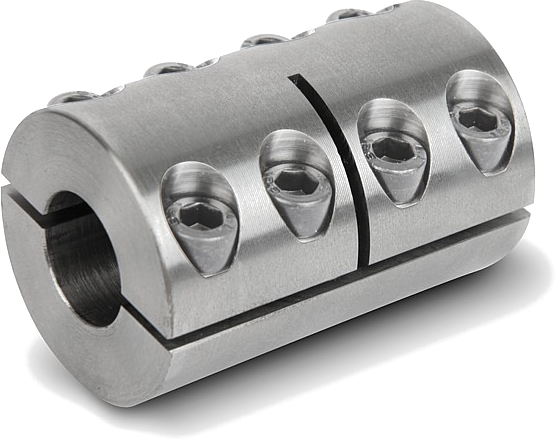
\includegraphics[width=0.68cm,height=0.6cm,keepaspectratio]{graphics/schalenkupplung.png} & Schalen- & \MKlvl{2}{klein--hoch} & \MKlvl{1}{klein--mittel} & \MKlvl{0}{keine} & \MKlvl{0}{keine} & \MKlvl{0}{keine} \\
  \hline
  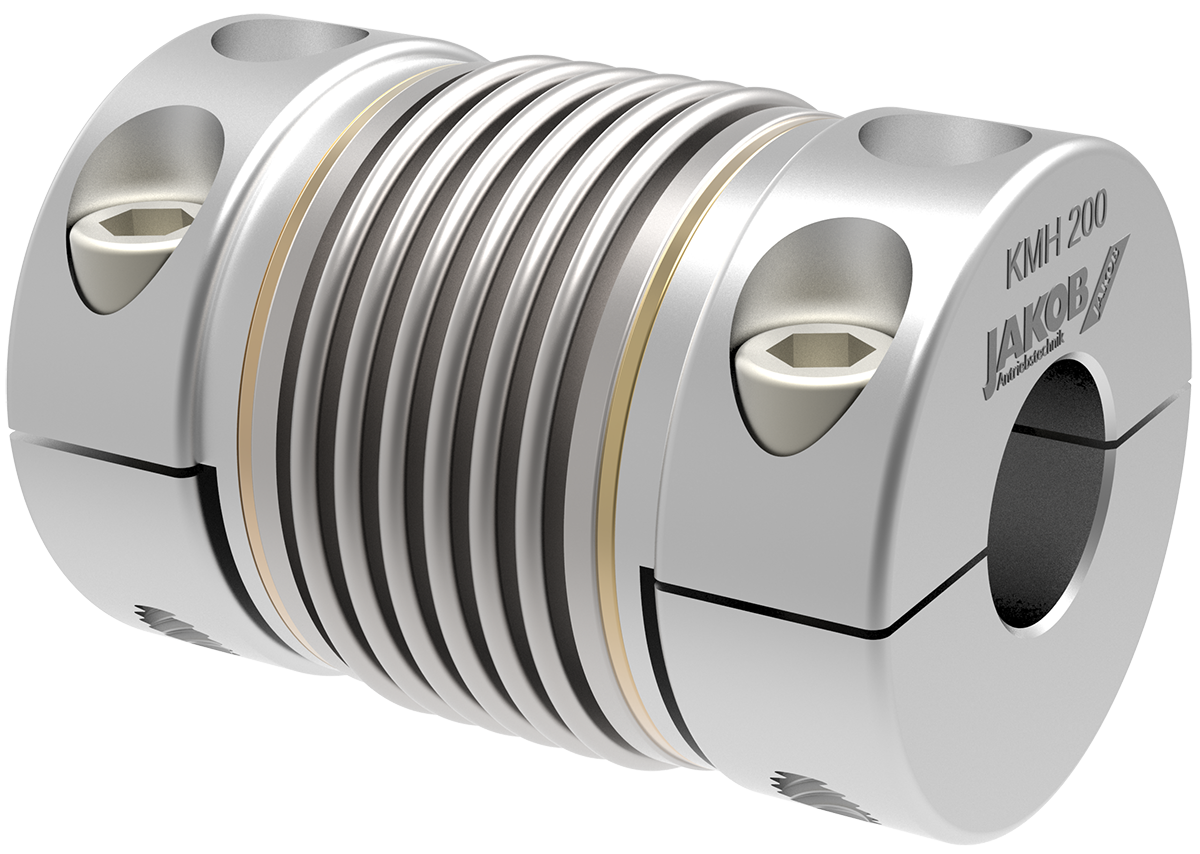
\includegraphics[width=0.68cm,height=0.6cm,keepaspectratio]{graphics/metallbalgkupplung.png} & Metall\-balg- & \MKlvl{3}{mittel--hoch} & \MKlvl{3}{mittel--hoch} & \MKlvl{3}{gut} & \MKlvl{3}{gut} & \MKlvl{4}{sehr gut} \\
  \hline
  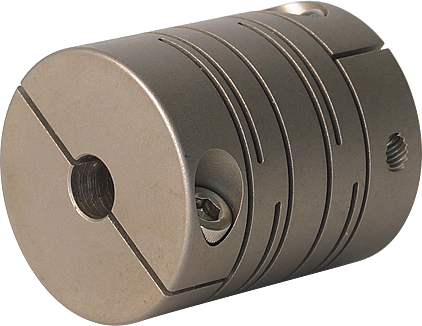
\includegraphics[width=0.68cm,height=0.6cm,keepaspectratio]{graphics/federstegkupplung.png} & Feder\-steg- & \MKlvl{1}{klein--mittel} & \MKlvl{3}{mittel--hoch} & \MKlvl{1}{kaum} & \MKlvl{3}{gut} & \MKlvl{3}{gut} \\
  \hline
  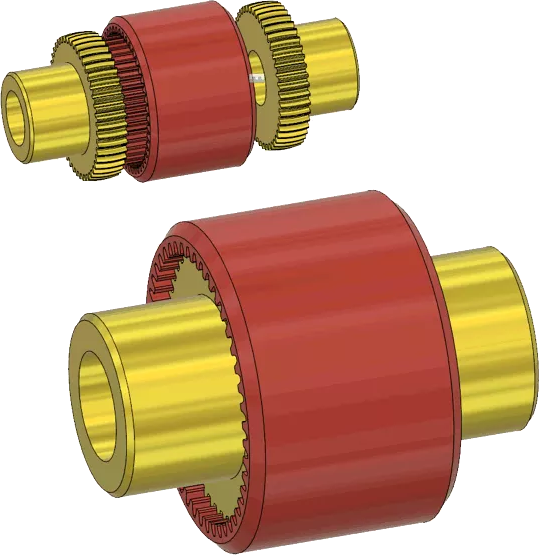
\includegraphics[width=0.68cm,height=0.6cm,keepaspectratio]{graphics/bogenzahnkupplung.png} & Bogen\-zahn- & \MKlvl{4}{hoch--\newline sehr~hoch} & \MKlvl{3}{mittel--hoch} & \MKlvl{3}{gut} & \MKlvl{4}{sehr gut} & \MKlvl{3}{gut} \\
  \hline
  \end{ZSFtablePlain}%
  \arrayrulecolor{black}}%
}

\newcommand{\ZSFKupplungenDrehelastischTabelle}{%
  {\setlength{\tabcolsep}{0.8pt}%
  \arrayrulecolor{black!35}%
  \begin{ZSFtablePlain}[\ZSFfontRel{-3bp}{0.3bp}]{|>{\columncolor{black!8}}Z{0.9}|>{\columncolor{black!8}}Z{1.42}|Z{0.98}|Z{0.95}|Z{0.9}|Z{0.9}|Z{0.95}|}
  \hline
  \ZSFheaderRow \ZSFhead{} & \ZSFhead{Kupplung} & \ZSFhead{Drehmom.} & \ZSFhead{Drehz.} & \multicolumn{3}{c|}{\ZSFhead{Versatz-Ausgleich}} \\
  \ZSFheaderRow \ZSFhead{} & \ZSFhead{} & \ZSFhead{} & \ZSFhead{} & \ZSFhead{axial} & \ZSFhead{radial} & \ZSFhead{winklig} \\
  \noalign{\global\arrayrulewidth=1.1pt}\hline\noalign{\global\arrayrulewidth=0.4pt}%
  \multicolumn{7}{|l|}{\cellcolor{white}\MKrfIcon{icon_drehelastisch}\ \textbf{Drehelastisch}{\color{black!60}: dämpft Stösse, nicht winkelsynchron}} \\
  \noalign{\global\arrayrulewidth=1.1pt}\hline\noalign{\global\arrayrulewidth=0.4pt}%
  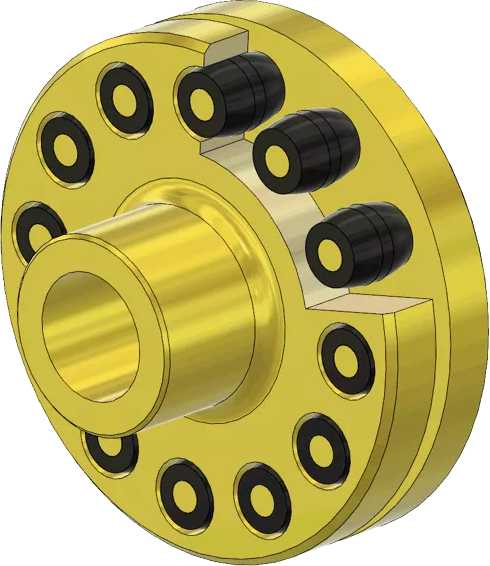
\includegraphics[width=0.68cm,height=0.6cm,keepaspectratio]{graphics/bolzenkupplung.png} & Bolzen- & \MKlvl{4}{hoch--\newline sehr~hoch} & \MKlvl{1}{klein--mittel} & \MKlvl{3}{gut} & \MKlvl{1}{kaum} & \MKlvl{3}{gut} \\
  \hline
  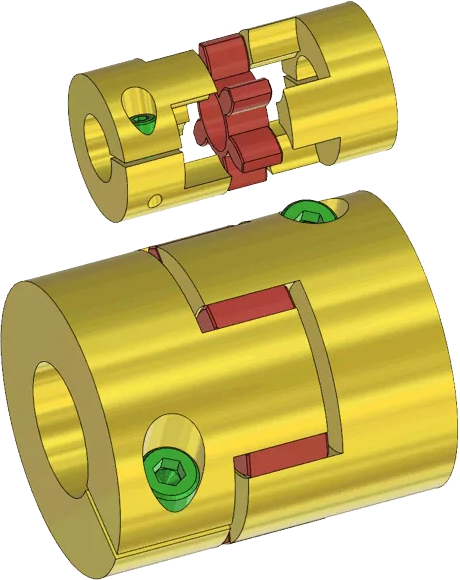
\includegraphics[width=0.68cm,height=0.6cm,keepaspectratio]{graphics/klauenkupplung.png} & Klauen- & \MKlvl{1}{klein--mittel} & \MKlvl{3}{mittel--hoch} & \MKlvl{3}{gut} & \MKlvl{1}{kaum} & \MKlvl{3}{gut} \\
  \hline
  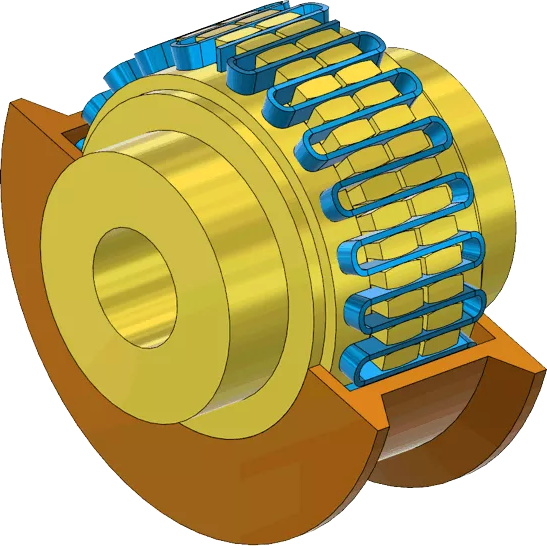
\includegraphics[width=0.68cm,height=0.6cm,keepaspectratio]{graphics/schlangenfederkupplung.png} & Schlangen\-feder- & \MKlvl{3}{mittel--hoch} & \MKlvl{1}{klein--mittel} & \MKlvl{3}{gut} & \MKlvl{3}{gut} & \MKlvl{3}{gut} \\
  \hline
  \end{ZSFtablePlain}%
  \arrayrulecolor{black}}%
}
